\subsection{Analyse von Temperaturfehlern}\label{apx:berechnung_temperaturfehler_interpolation}
\subsubsection{Vergleich von Modellierungsmöglichkeiten}
Im Folgenden werden die in Kapitel \ref{sec:temp_messung_code_conversion} angesprochenen Techniken miteinander verglichen, um anschliessend eine Approximationsmethode bestimmen zu können, welche definitv umgesetzt wird.\lb
Zuerst werden die folgenden Ansätze zur Umschreibung des Widerstandwertes im Temperaturbereich von -50...\SI{200}{\celsius} verfolgt:
\begin{itemize}[noitemsep,topsep=3pt]
	\item Linearisierung der Funktion.
	\item Umschreibung der Funktion durch quadratische Funktion.
	\item Umschreibung der Funktion durch kubische Funktion.
	\item Anwendung eines \ac{LUT} mit den Widerstandswerten im Abstand von \SI{1}{\celsius} mit Interpolation in \SI{0.1}{\celsius} zwischen den Werten.
\end{itemize}\vspace{11pt}
Die Berechnungen werden in Microsoft's Excel durchgeführt, die Funktionen zu der Linearisierung sowie den Polynomen werden ebenfalls mit Excel generiert. Mehr Informationen zu den Berechnungen sind direkt aus dem Excel-Sheet zu entnehmen.\lb
In einem ersten Schritt wird mit den resultierenden Funktionen der verschiedenen Methoden jeweils die Abweichung zum Soll-Widerstandswert berechnet. So können die verschiedenen Methoden auf ihre Eignung eingestuft werden. Die folgende Graphik zeigt den Widerstandsfehler in \SI{}{\ohm} in Abhängigkeit der Temperatur.
\begin{figure}[H]
	\centering
	\captionsetup{justification=centering}
	\includegraphics[width=1.0\linewidth]{anhang/abb/rtd_fehlerbetrachtung}
	\caption{Vergleich des Widerstandsfehlers bei unterschiedlichen Approximationstechniken}
	\label{fig:widerstandsfehler_rtd_vergleich}
\end{figure}
Aus diesen Abklärungen geht hervor, dass mit einem \ac{LUT} die bestmögliche Genauigkeit im Vergleich zu den restlichen Methoden erzielt werden kann. Im folgenden Unterkapitel wird der effektive Temperaturfehler unter Anwendung eines Lookup Tables berechnet. \newpage
\subsubsection{Fehlerberechnung unter Anwendung eines Lookup Tables}
Dieses Kapitel beschreibt das Vorgehen und die Überlegungen zur Berechnung des Temperaturfehlers für den Ansatz, dass in einem \ac{LUT} die \ac{ADC} Output Codes für die Temperaturwerte im Abstand von \SI{1}{\celsius} abgelegt sind. Desto kleiner der Abstand gewählt wird, desto kleiner wird der entstehende Fehler, jedoch steigt damit auch der Speicheraufwand und Suchaufwand im \ac{LUT} linear an. Die Berechnungen wurden in einem Matlab-Skript durchgeführt. Dabei wurde zuerst der erwartete Output Code des \ac{ADC} für eine Temperatur von \SI{0}{\celsius} berechnet:
\begin{equation}
\mathrm{ADC_{Output\ Code}}= \dfrac{R_0 \cdot \mathrm{IDAC}}{\mathrm{LSB}} = \dfrac{\SI{100}{\ohm} \cdot \SI{500}{\micro\ampere}}{\SI{2.86}{\micro\volt}} = 17476\mathrm{d}
\end{equation}
Im Anschluss wurde von diesem dezimalen Wert aus bis zum maximalen ADC-Wert von $2^{15}-1=32768\mathrm{d}$ der auf Basis der \ac{LSB} zu erwartende Spannungsabfall über dem \ac{RTD} berechnet. Da der Messstrom IDAC bekannt ist, lässt sich der dazugehörende Widerstandswert berechnen. Mit der Formel \ref{equ:cvt_umgestellt_temp} kann anschliessend wiederum der dazugehörige Temperaturwert berechnet werden. Diese Werte gelten als Basis für den späteren Vergleich mit den Resultaten, die mit der Interpolation berechnet werden.\lb
Bei der wird ein \ac{LUT} für die erwarteten \ac{ADC} Output Codes nach folgendem Schema berechnet:
\begin{equation}
\dfrac{R_{RTD}(T) \cdot IDAC}{LSB} \hspace{8mm} \mathrm{für: } \ T=\{0, 1, 2, ...\} 
\end{equation}
Anschliessend wird iterativ alle im \ac{ADC} Output Code Werte "'$ADC_{dec}$"' im gesamten Bereich der folgende Algorithmus angewendet:
\begin{itemize}[noitemsep,topsep=5pt]
	\item $\mathrm{LUT_{dec}}$ := erster Wert aus dem \ac{LUT}, der gleich gross oder grösser als der aktuelle \ac{ADC} Output Code ist. Dazu wird ein Index $n$ ermittelt für den Zugriff auf das $\mathrm{LUT_{dec}}$-Array.
	\item $\mathrm{d_{dec}}$ := Unterschied zwischen "'$\mathrm{ADC_{dec}}$"' zu $\mathrm{LUT_{dec}}$ (entspricht dem delta x, womit im Anschluss 
	\item slope := 1 / $\mathrm{d_{dec}}$ (Temperaturanstieg in Grad Celsius pro zusätzlichen decimalen Wert)
	\item dT := "'$\mathrm{ADC_{dec}} \cdot \mathrm{slope}$"' (Temperaturunterschied vom Wert im \ac{LUT})
	\item baseT := n (Entspricht dem Index des $\mathrm{LUT_{dec}}$-Arrays)
	\item Ti := baseT + dT (Entspricht der Interpolierten Temperatur)
\end{itemize}
Bildlich dargestellt handelt es sich um folgende Vorgehensweise, dargestellt für einen kleinen Wertebereich von \SI{0}{\celsius} bis \SI{3}{\celsius}. Für negative Temperaturwerte muss der LUT lediglich ergänzt werden, zusätzlich muss ein Offset für die Bestimmung der Basistemperatur "'baseT"' addiert werden. Es ist davon auszugehen, dass der Fehler für negative Temperaturen im selben Grössenbereich liegt. 
\begin{figure}[H]
	\centering
	\includegraphics[width=0.9\linewidth]{abb/lut_funktionsweise}
	\caption{Funktionsweise des LUT am Beispiel eines Inputs von 17671}
	\label{fig:temperatur_lut_funktionsweise}
\end{figure}
Der Fehler ergibt sich anschliessend aus der Differenz zwischen der Solltemperatur mit perfekter Auflösung (für jeden \ac{ADC} Output Code die Temperatur hinterlegt) und den interpolierten Temperaturwerten (Ti).\lb
Aus den Berechnungen im Matlab Skript resultiert die folgende Graphik. \begin{figure}[H]
	\centering
	\captionsetup{justification=centering}
	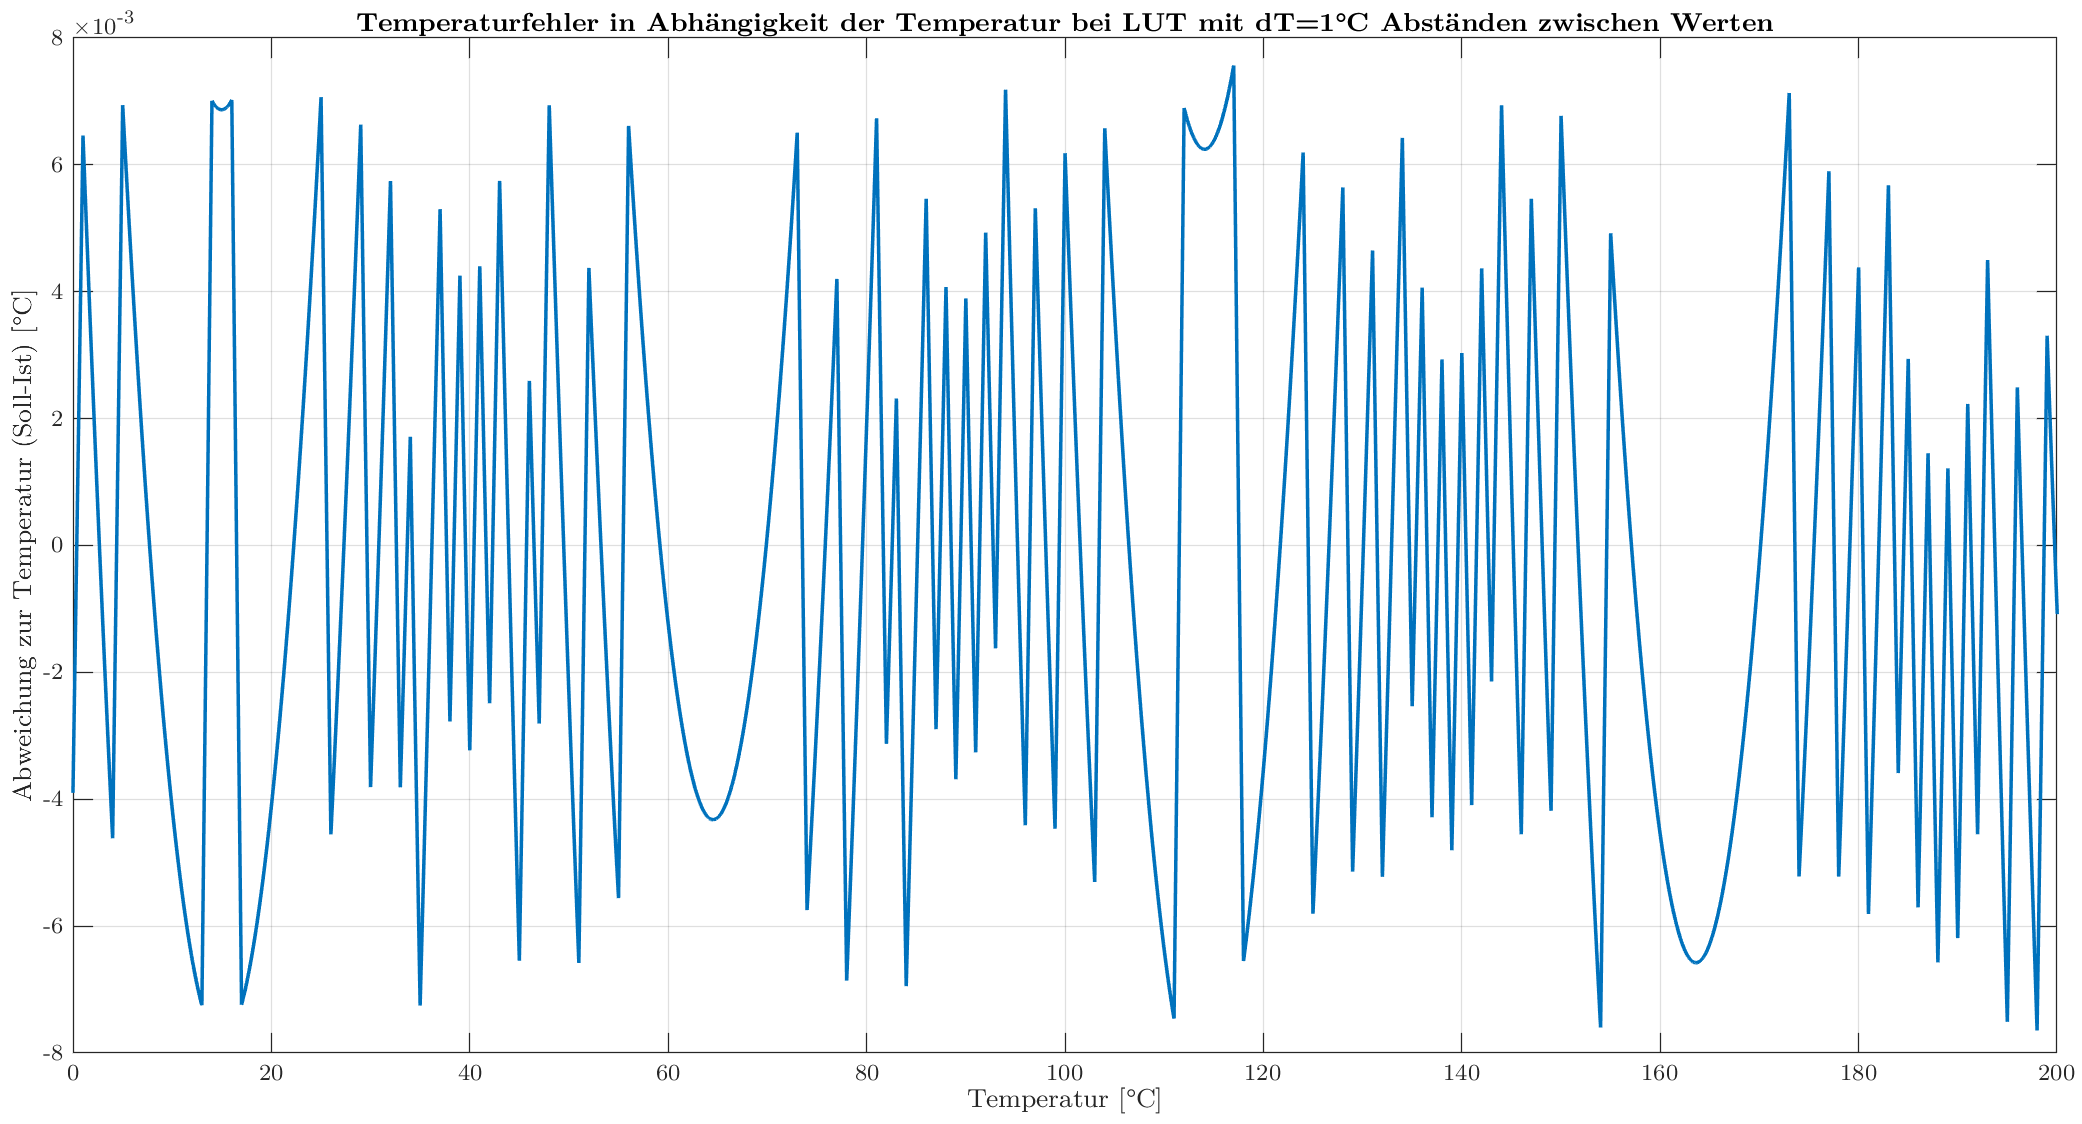
\includegraphics[width=1.0\linewidth]{anhang/abb/temperaturfehler_interpolation}
	\caption{Zu erwartender Temperaturfehler bei einem LUT mit Werten im Abstand von \SI{1}{\celsius} und einer Interpolation über den positiven Temperaturbereich}
	\label{fig:temperaturfehler_interpolation_lut}
\end{figure}